\documentclass[chapterprefix=false,a4paper,12pt]{report}
\usepackage[left=2.5cm,right=2.5cm,top=2cm,bottom=3cm]{geometry}
\usepackage{graphicx}
\usepackage{verbatim}
\usepackage{latexsym}
\usepackage[toc]{appendix}
\usepackage{titlesec}
\usepackage{longtable}
\usepackage{array}
\usepackage{float}
\usepackage{syntax}
\usepackage{amsmath}

\titleformat{\chapter}[block]
   {\normalfont\huge\bfseries}{\chaptertitlename\ \thechapter}{20pt}{\Huge}

\pagestyle{empty}

\setlength{\parskip}{0em}
\setlength{\parindent}{0em}

\makeatletter
\def\submitdate#1{\gdef\@submitdate{#1}}
\def\degree#1{\gdef\@degree{#1}}
\def\studentid#1{\gdef\@studentid{#1}}
\def\supervisor#1{\gdef\@supervisor{#1}}

\def\maketitle{
    
  \begin{titlepage}{
    
    \centering{
    
\includegraphics[width=0.25\columnwidth]{images/sussex-logo.png}} \par
    
    \vskip 0.5in \par 
    \LARGE {\textbf{\@title}}
    
    \vskip 0.5in \par
    \normalsize {Submitted \@submitdate, in partial fulfillment of \\ the conditions for the award of the degree \bf{\@degree}.}

  }
  \vskip 0.3in \par
  \large {\bf \@author} \par
  \large {\bf \@studentid}
  
  \vskip 0.3in \par
  \large {\bf Supervised by \@supervisor}
  \vskip 0.3in \par
  \normalsize { School of Computer Science \par
  University of Sussex}

  \vskip 0.5in \par
  \normalsize {I hereby declare that this dissertation is all my own work, except as indicated in the text: }

  \vskip 0.2in 
  \normalsize {Signature: Samuel Withey}
  
  \vskip 0.1in
  \normalsize {Date: 09/06/2020}
  
  \vskip 0.4in \par
  \normalsize {The report may be freely copied and distributed provided the source is acknowledged. I hereby give permission for a copy of this report to be loaned out to students in future years.}
  
  \end{titlepage}
}

\def\titlepage{
  \newpage
  \centering
  \linespread{1}
  \normalsize
  \vbox to \vsize\bgroup\vbox to 9in\bgroup
}
\def\endtitlepage{
  \par
  \kern 0pt
  \egroup
  \vss
  \egroup
  \clearpage
}

\def\abstract{
  \begin{center}{
    \large \bf Abstract}
  \end{center}
  \small
  \normalsize
}
\def\endabstract{
  \par
  \clearpage
}

\newenvironment{acknowledgements}{
  \cleardoublepage
  \begin{center}{
    \large \bf Acknowledgements}
  \end{center}
  \small
  \normalsize
}{\cleardoublepage}
\def\endacknowledgements{
  \par
}

\def\preface{
    \pagenumbering{roman}
    \pagestyle{plain}
}

\def\body{
	
    \cleardoublepage    
    \clearpage
    \pagestyle{plain}
    \tableofcontents
    \pagestyle{plain}
    \cleardoublepage
    \pagenumbering{arabic}
}

\makeatother

\newcolumntype{P}[1]{>{\arraybackslash}p{#1}}
\newcolumntype{C}[1]{>{\centering\arraybackslash}m{#1}}

\begin{document}

\title{A Domain Specific Language for Twitter Bots}

\author{Samuel Withey}
\submitdate{June 2020}
\degree{BSc Computer Science}
\studentid{164574}
\supervisor{Professor Ian Wakeman}

% \normallinespacing
\maketitle

\preface
\addcontentsline{toc}{chapter}{Abstract}

\begin{abstract}

The increase of users on social media platforms provides a new way for users and brands to connect with their audiences. This report explores the concept of designing, building and implementing a lightweight language to automate social media content and interactions through Twitter bots. Using Twitter bots is often outside the competence level of the typical Twitter user. The project aims to provide a novel solution to connect the average Twitter user with the features and automation of Twitter bots. The solution is achieved by a domain specific language using the latest parser generator tools to bridge the gap of the Twitter API to the novice user. The project provides a web-application using modern web-frameworks to provide a user interface to interact with the language and to make the project accessible to all users.

\end{abstract}
\addcontentsline{toc}{chapter}{Acknowledgements}

\begin{acknowledgements}

I would first like to thank my supervisor, Ian Wakeman, whose expertise was invaluable and support was greatly appreciated throughout the entire process and a challenging second term. \newline \par

In addition I would like to thank my parents, who have provided emotional support and a sympathetic ear throughout the entire duration of the course and key moments of the final year project.

\end{acknowledgements}

\body
\renewcommand{\chaptername}{}

\chapter{Introduction}

In January 2019, it was reported that there were 3.484 billion worldwide active users across all social media platforms. This rapid social paradigm shift has transformed consumer behaviour and social interaction through online social platforms which allow instantaneous direct communication. This has provided unbounded limitations for brands to connect and engage directly with their audiences.

\section{Motivation}

The motivation of the project is finding a unique solution around managing and automating social media content on Twitter. This is because of the limited functionality that the standard Twitter web page provides, with a lack of automation it makes managing large amounts of content and intricate tasks.

\section{Aims}

The aim of the project is to provide a solution to the limited functionality of Twitter by bridging the gap between the novice user and the Twitter API. This will be achieved by designing and implementing a domain specific language and an interpreter. This allows a lightweight language to provide the user with the core functionality of what can be achieved on Twitter with added functionality of the Twitter API including scheduling and automating content.

\section{Domain Specific Languages}

Domain specific languages are optimised for a given class of problems called a domain.  It is based on abstractions that are closely aligned with the domain for which the language is built and a domain specific languages syntax is suitable for expressing these abstractions concisely. This differs from general-purpose languages which are used by programmers to instruct computers. General-purpose languages are Turing complete, which means they can be used to implement anything that is computable by a Turing machine. \\

An advantage of using a domain specific language is that it is another layer of abstraction. Notation can be defined that expresses the abstractions concisely and makes interacting with programs easy and efficient. This is important for the project as the domain specific language can be used by non-programmers. It provides a clean level of abstraction that moves away from general-purpose languages and API’s which non-programmers are not competent enough to use and allows them to work with a language closely aligned with the domain they work in. This is a key solution to the problem area as it abstracts the complexity of using API’s by creating a language which is syntactically simpler than a general purpose language and can be used by non-programmers which is the target user for the system. \\

For the domain specific language to execute it requires an interpreter or compiler. When text is interpreted, it is parsed and the result from the program is produced in a single process. \\

A parser is the processing of structuring a text according to a given grammar. The parser will generate a syntax/parse tree which is a data structure which precisely shows how various segments of the program text are to be viewed in terms of the grammar. A grammar or context-free grammar are the formalism for describing the structure of programs in a programming language by describing the syntactic structure. Since the semantics of a language is defined in terms of the syntax, the context-free-grammar is also instrumental in the definition of the semantics. \\
\chapter{Background}

\section{Domain Specific Languages}

A general-purpose programming language is designed for writing software in a variety of application domains. It is used by programmers to instruct computers by implementing any program that is computable by a Turing machine \cite{DslEngineering2013}. Conversely, a domain specific language is optimised for a given class of problems called a domain.  The syntax is based on abstractions that are closely aligned with the domain for which the language is built. A domain specific languages syntax is suitable for expressing these abstractions concisely \cite{DslEngineering2013}. A notable example of a domain specific language is Structured Query Language (SQL), designed for managing data held in a relational database management system. \newline \par

There are many advantages of using a domain specific language over a general-purpose language. The main advantage is that the domain specific language provides an additional layer of abstraction for the user. Notation can be defined that expresses the abstractions concisely and makes interacting with programs efficient and straightforward. This notation allows users of the domain specific language to have less experience with programming due to the limited scope of the language. It provides a clean level of abstraction that moves away from general-purpose languages and API’s which non-programmers are not competent enough to use. This abstraction allows non-programmers to work with a language closely aligned with the domain they work in \cite{DslEngineering2013},  yielding programs that are easy to understand, reason about, and maintain \cite{685738}. This is a crucial solution to the problem area as it abstracts the complexity of using API’s by creating a language which is syntactically simpler than a general-purpose language. \newline \par

Another advantage of using a domain specific language is their ability to be analysed and maintained. Due to the limited complexity of domain specific languages, certain properties such as termination can be determined, unlike general-purpose languages. These properties allow the domain specific language to be safer, often throwing less and more meaningful errors, which can be useful when dealing with critical services. For a domain specific language to execute it requires an interpreter or compiler.

\section{Interpreter}

For the execution and implementation of a language, another program or application is required to read the language and react to the phrases and input symbols it discovers. The program or application to execute this task is the interpreter. To execute the input, the interpreter must react to the valid sentences, phrases and sub-phrases of a particular language. The interpreter needs to be able to recognise phrases and identify the valid components of the phrase and differentiate it from other phrases \cite{parr2013definitive}. \newline \par

After the recognition of each phrase in a program, the interpreter will execute precompiled application specific code based on the phrase and valid components of the input \cite{hudak1997domain}. Unlike compilers, interpreters do not require code generation to machine language. Programs that recognise languages are called parsers, and this process is broken down into two stages, lexical analysis and parsing.

\section{Lexer}

Lexical analysers, often referred to as lexers, are programs which read the input stream of characters making up the source program, groups the characters into meaningful sequences called lexemes and produce as output a sequence of tokens for each lexeme \cite{aho2003compilers}. Tokens may be considered the building blocks of the language as it is more convenient to process a source program as a sequence of tokens rather than a string of characters. Tokens consist of two pieces of information, the token type, used to identify the lexical structure and the text matched for that token by the lexer in the form $\langle \textit{token-name}, \textit{attribute-value} \rangle$ \cite{aho2003compilers}. In general-purpose languages such as Java, examples of token types are int (integers), double (floating-point numbers). Another task the lexer performs is stripping out comments and white space in a source program.\newline \par

Lexers do not check the grammatical syntax of the language, as it will not check if the tokens are used in the wrong combination and will only produce a list of tokens. The list of tokens is passed to the subsequent phase, parsing, which is the process of identifying if an input is syntactically correct. 

\section{Parser}

A parser is a program to recognise the sentence structure of an input which is the process of structuring an input text according to a given grammar. The parser uses the token types of the tokens produced by the lexical analyser to produce a tree-like intermediate representation that depicts the grammatical structure of the token stream \cite{aho2003compilers}.

\subsection{Grammar}

A grammar is a formalism for describing the syntactic structure of programs in a programming language. A grammar describes how to form grammatical strings from a language's alphabet that are valid according to the syntax of the language by a set of production rules \cite{meduna2014formal}. A grammar derives strings by beginning with the start symbol and repeatedly replacing a nonterminal by the body of production for the nonterminal. The terminal strings that can be derived from the start symbol form the language defined by the grammar \cite{aho2003compilers}. A grammar does not describe the meaning of the strings in any given context and only describes their form.\newline \par

A context-free grammar is a grammar in which the left-hand side of every production rule consists of only a single nonterminal symbol in the form $ A \rightarrow \alpha$ where $A$ is a single nonterminal symbol, and $\alpha$ is a string of terminals and/or nonterminals \cite{aho1971translations}. A grammar is context-free when the production rules can be applied regardless of the context of a nonterminal. Since the semantics of a language is defined in terms of the syntax, the context-free-grammar is also instrumental in the definition of the semantics \cite{grune2012modern}. \newline \par

The formal definition of a context-free grammar G is defined by a four-tuple $G = (V, \varSigma, P, S)$, where $V$ and $\varSigma$ are disjoint finite sets of non-terminals and terminals which make up the content of the sentence \cite{aho1971translations}. $S$ is the start variable/symbol, used to represent the whole sentence or program and is an element of V. $P$ is a finite list of productions or rewrite rules of the form $ A \rightarrow \alpha$, where $A$ is in $V$ and $\alpha$ in $(V\cup\varSigma)^\ast$ \cite{backus1960report}.

\subsubsection{Left-recursive Grammar}

In a context-free grammar G, if there is a production in the form $X \rightarrow Xa$ where $X$ is a non-terminal and $a$ is a string of terminals, it is called a left recursive production. The grammar having a left recursive production is called a left recursive grammar, and this grammar would fall into infinite recursion when executed \cite{moore2000removing}.

\subsection{Parse Tree}

The parser will generate a syntax/parse tree which is a data structure that precisely shows how various segments of the program text and component phrases are to be recognised in terms of the grammar. Parse trees are a useful data structure as they contain complete information about how the parser grouped symbols into phrases and can easily be traversed by programmers \cite{parr2013definitive}. The construct of a parse-tree can be made by taking a derivational view, in which productions are treated as rewriting rules. The initiation of the derivation starts with the start symbol, and each rewriting step replaces a nonterminal by the body of one of its productions. An example of a parse tree is if a nonterminal $A$ has a production $A \rightarrow XYZ$, then a parse tree may have an interior node labelled A with three child nodes, labelled from left to right $X$, $Y$ and $Z$ \cite{aho2003compilers}. 

\begin{figure}[H]
  \centering
  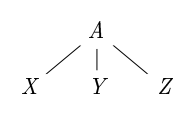
\includegraphics[width=0.25\textwidth]{images/parse-tree2.PNG}
  \caption{Example Parse tree \cite{aho2003compilers}}
\end{figure}

A formal definition of a parse tree according to a context-free grammar is a tree with the following properties \cite{aho2003compilers}:
\begin{itemize}
    \item The root node is labeled by the start symbol.
    \item Each leaf node is labeled by a terminal or by $\epsilon$.
    \item Each interior node is labeled by a nonterminal.
\end{itemize}

\begin{figure}[H]
  \centering
  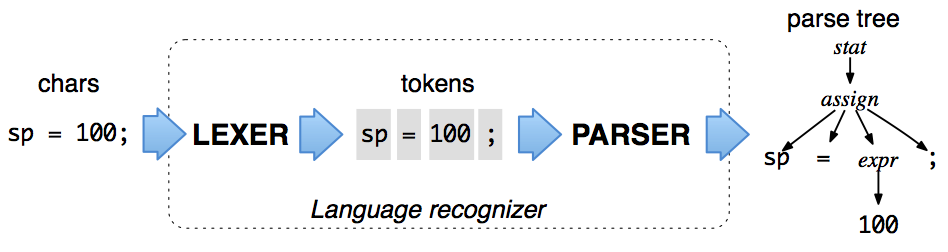
\includegraphics[width=1\textwidth]{images/antlr2.png}
  \caption{Data flow of a lexer and parser \cite{parr2013definitive}}
\end{figure}

\subsection{Top-down Parsing}

A top-down parser uses a context-free grammar $G$ and works on an input string $w$. It verifies that w is syntactically correct by constructing the derivation tree for $w$ in a top-down way. A derivation of an input for a grammar is a sequence of grammar rule applications that transform the start symbol into the string. The derivation proves that the input belongs to the language of the grammar. The derivation reads input string $w$ from left to right, and the parser starts at the tree node and proceeds down towards the frontier denoted by $w$. A LL grammar is a grammar that can be parsed by an LL parser. The first L stands for left-to-right scan of the input string $w$ and the second L means that the parser simulates the leftmost derivation of $w$ \cite{meduna2014formal}.
\chapter{Professional Considerations}

The nature of the project using social media automation results in a large array of ethical and professional considerations. The aims and motivations for the project are for individuals and brands to allow more automation and freedom to manage and publish their social media content however the project could be used in a variety of negative ways. Examples of real world negative ethical consequences of social media automation are spam, harassment, spreading false information, troll armies and influencing content reach and impressions. \newline \par

Mitigating the risk of the tool being used for negative consequences is an intricate task to be implemented into the project. To access and interact with the Twitter API, users must have authorised consumer keys and access tokens by Twitter. This allows the project to be an extension of the Twitter API by only allowing users who have been pre-authorised to access the Twitter API. If the user of the tool violates the Developer Agreement and Policy \cite{DeveloperPolicy}, their access to the Twitter API would be revoked and the user would not be able to use the tool. \newline \par

Another ethical consequence of social media automation is spam. The Twitter API imposes rate limits, which is a per-user basis of how often users can invoke API methods. If these limits are exceeded, a time penalty will be added to the user and this is a way to combat spam. Since the implementation of the domain specific language does not contain any direct looping or recursion, it is not necessary to directly implement rate-limits into the standard functionality of the domain specific language. The rate limits have been imposed on the automated bot scripts to combat spam and to stay within the Twitter Developer Agreement and Policy \cite{DeveloperPolicy}. Tweepy, a Python library used for accessing the Twitter API in the project has its own functionality to restrict spam. When making posts, Tweepy requires each post to be unique. If a post is not unique, a duplicate error will be raised and the post will not be posted.

\section{BSC Code of Conduct}

Ethical standards governing the conduct of computing professionals in the UK are set out in the Code of Conduct published by BCS - The Chartered Institute for IT. The project adheres to all standards set by the code of conduct. Section 1.a, Public Interest, is an important standard as the use of automation could disregard the well-being of others and the project adheres to this standard through built in rate-limits. All of the source code for the project will be open source and publicly available on GitHub to uphold Section 4, Duty to Profession. This will be in direct accordance with section 4.f, to encourage and support fellow members in their professional development.

\chapter{Requirements Analysis}

The system is designed to be used by any user, brand or agency who are competent social media users. To understand the needs of users and to what extent their current solutions meet their needs, interviews were conducted with InCrowd. \newline \par

InCrowd is a company based in London and Brighton who provide intuitive sports technology to help brands engage with their audiences. The interviewees who work for InCrowd work in the Marketing team. Person 1 solely uses Twitter and native Twitter tools in their day to day job role. Person 2 works in the Business to Business (B2B) marketing team and focuses on using Twitter and Linkedin to achieve this role. Both interviewees use the tools and applications of the native platform but have used other industry-standard social media management tools to automate and schedule content in previous job roles. \newline \par

Functional and Non-Functional requirements are devised from the interviews conducted with InCrowd. The outcome of the requirements analysis is combined with the knowledge of the Twitter API and the overall goals and aims of the project. 

\section{Functional Requirements}

\begin{longtable}{|>{\centering}C{1.7cm}|P{7cm}|C{3.7cm}|} \hline
    {Reference} & {Description} & {Mandatory/Desirable} \\ \hline
    F1 & The system shall provide the basic functionality of what actions can be completed by a human on Twitter which can be configured and executed by the domain specific language. This functionality includes login, post tweets, reply to tweets, retweet tweets, like tweets and follow users. & Mandatory \\ \hline 
    F2 & The system shall allow scheduling for content on Twitter through the domain specific language. & Mandatory \\ \hline 
    F3 & The system shall provide the functionality to automate favouriting and retweeting tweets based on keywords through the domain specific language. & Mandatory \\ \hline
    F4 & The system shall provide the functionality to automate responding to tweets based on keywords through the domain specific language. & Mandatory \\ \hline
    F5 & The system should provide the functionality to automate direct messaging to users based on keywords through the domain specific language. & Desirable \\ \hline
    F6 & The system should retrieve a list of relevant content from other users on the platform based on a customisable input such as keywords and hashtags. & Desirable \\ \hline
    F7 & The system should provide a list of suggested accounts to follow based on inputs such as keywords and hashtags. & Desirable \\ \hline
    F8 & The system should provide the ability to customise analytical reports within a given time frame. & Desirable \\ \hline
    F9 & The system should provide a web interface to display customisable Twitter feeds. & Desirable \\ \hline
    F10 & The system should provide a web interface to display scheduled Twitter posts and content. & Desirable \\ \hline
    F10 & The system should be deployed using cloud web-services. & Desirable \\ \hline
\end{longtable}
    
\section{Non-Functional Requirements}

\begin{longtable}{|>{\centering}C{1.7cm}|P{7cm}|C{3.7cm}|}  \hline
    {Reference} & {Description} & {Mandatory/Desirable} \\ \hline
    NF1 & The domain specific language shall run on Windows, Mac and Linux Operating Systems. & Mandatory \\ \hline
    NF2 & The domain specific language shall be programmed using Python 3 and use ANTLR4 toolkit. & Mandatory \\ \hline
    NF3 & The interpreter shall run on Windows, Mac and Linux Operating Systems. & Mandatory \\ \hline
    NF4 & The interpreter shall be programmed using Python 3 and use ANTL4 toolkit. & Mandatory \\ \hline
    NF5 & The web application shall run on all latest browsers. & Desirable \\ \hline
    NF6 & The web application shall be programmed using Python 3 and Django Web Framework. & Desirable \\ \hline
    NF7 & The web application shall use Django's user login system to provide security for the web application through user authentication. & Desirable \\ \hline
    NF8 & The web application shall be deployed using AWS. & Desirable \\ \hline
\end{longtable}
\setlength{\grammarparsep}{2pt plus 1pt minus 1pt} % increase separation between rules
\setlength{\grammarindent}{12em} % increase separation between LHS/RHS
\chapter{Design}
\section{UML}
UML designs assist with the visualisation of the requirements analysis, and it demonstrates the functionality and user interactions with the system. The UML designs include the full scope of the project. The full scope includes both functional and non-functional mandatory and desirable requirements and the broader scope of the aims and objectives of the project.

\subsection{Use Case Diagram}

A use case diagram is a representation of a user's interaction with the system that shows the relationship between the user and the different use cases in which the user is involved. The use-case diagrams are split to demonstrate the users' interactions with the domain specific language and the interaction of the web-application.
\begin{figure}
  \centering
  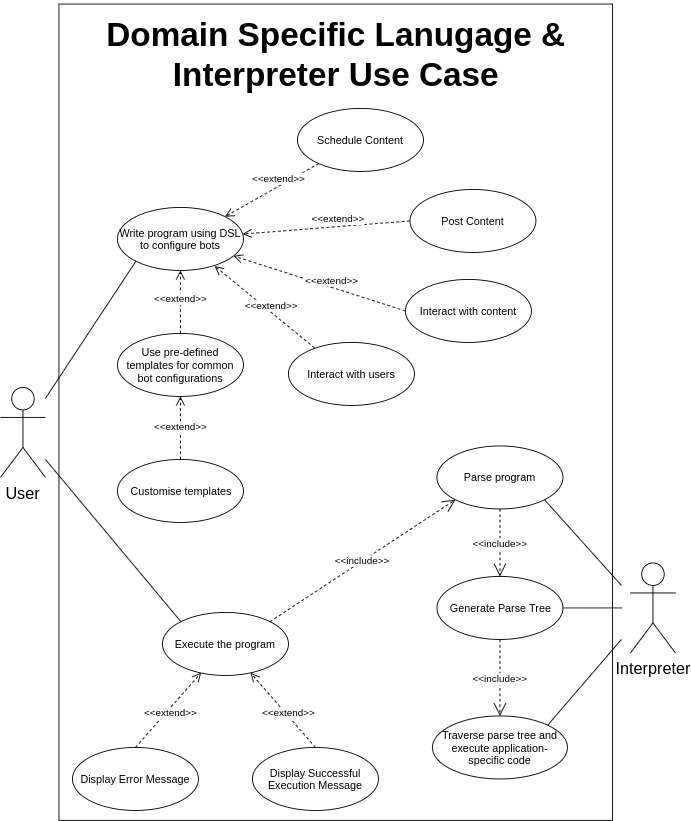
\includegraphics[width=0.9\textwidth]{images/usecasedsl.png}
  \caption{UML Use Case Diagram for DSL and Interpreter}
\end{figure}

\begin{figure}[H]
  \centering
  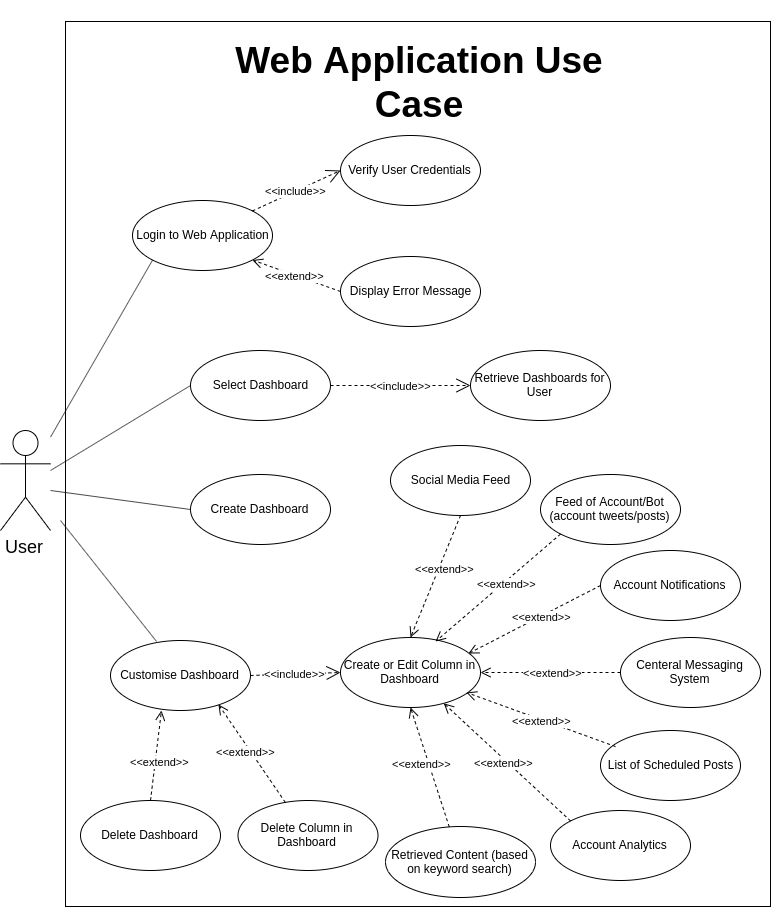
\includegraphics[width=0.9\textwidth]{images/usecasewebapp-2.png}
  \caption{UML Use Case Diagram for Web Application}
\end{figure}

\subsection{High-Level Domain Model}

The high-level domain model is a conceptual model of the domain that incorporates both behaviour and data. The domain model is a system of abstractions that describes selected aspects of a sphere of knowledge, influence or activity. The high-level domain model in figure 5.3 represents how the user interacts with the system and how the different components of the system are incorporated and interact with each other.

\begin{figure}[H]
  \centering
  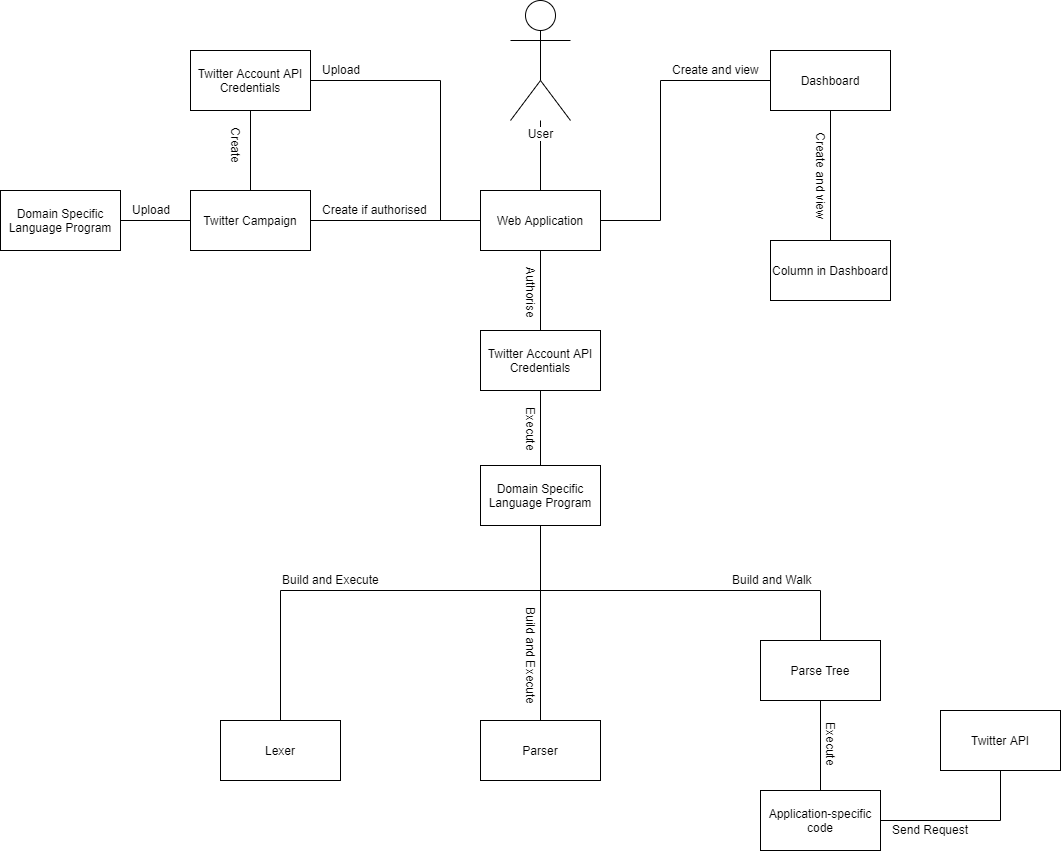
\includegraphics[width=1\textwidth]{images/high-level-domain.png}
  \caption{High-Level Domain Model}
\end{figure}

\subsection{Software Patterns}

The outcome of the high-level domain model loosely represents a conventional model-view-controller architecture. The model-view-controller architecture bases itself on three components, the model, the view and the controller. The model is the central component which usually reflects real-world objects and is used to store raw data. The view is a representation of the model to the user. The controller acts as a liaison between the model and the view and accepts user input, updates the model and produces an output for the view \cite{deacon2009model}. 

\begin{figure}[H]
  \centering
  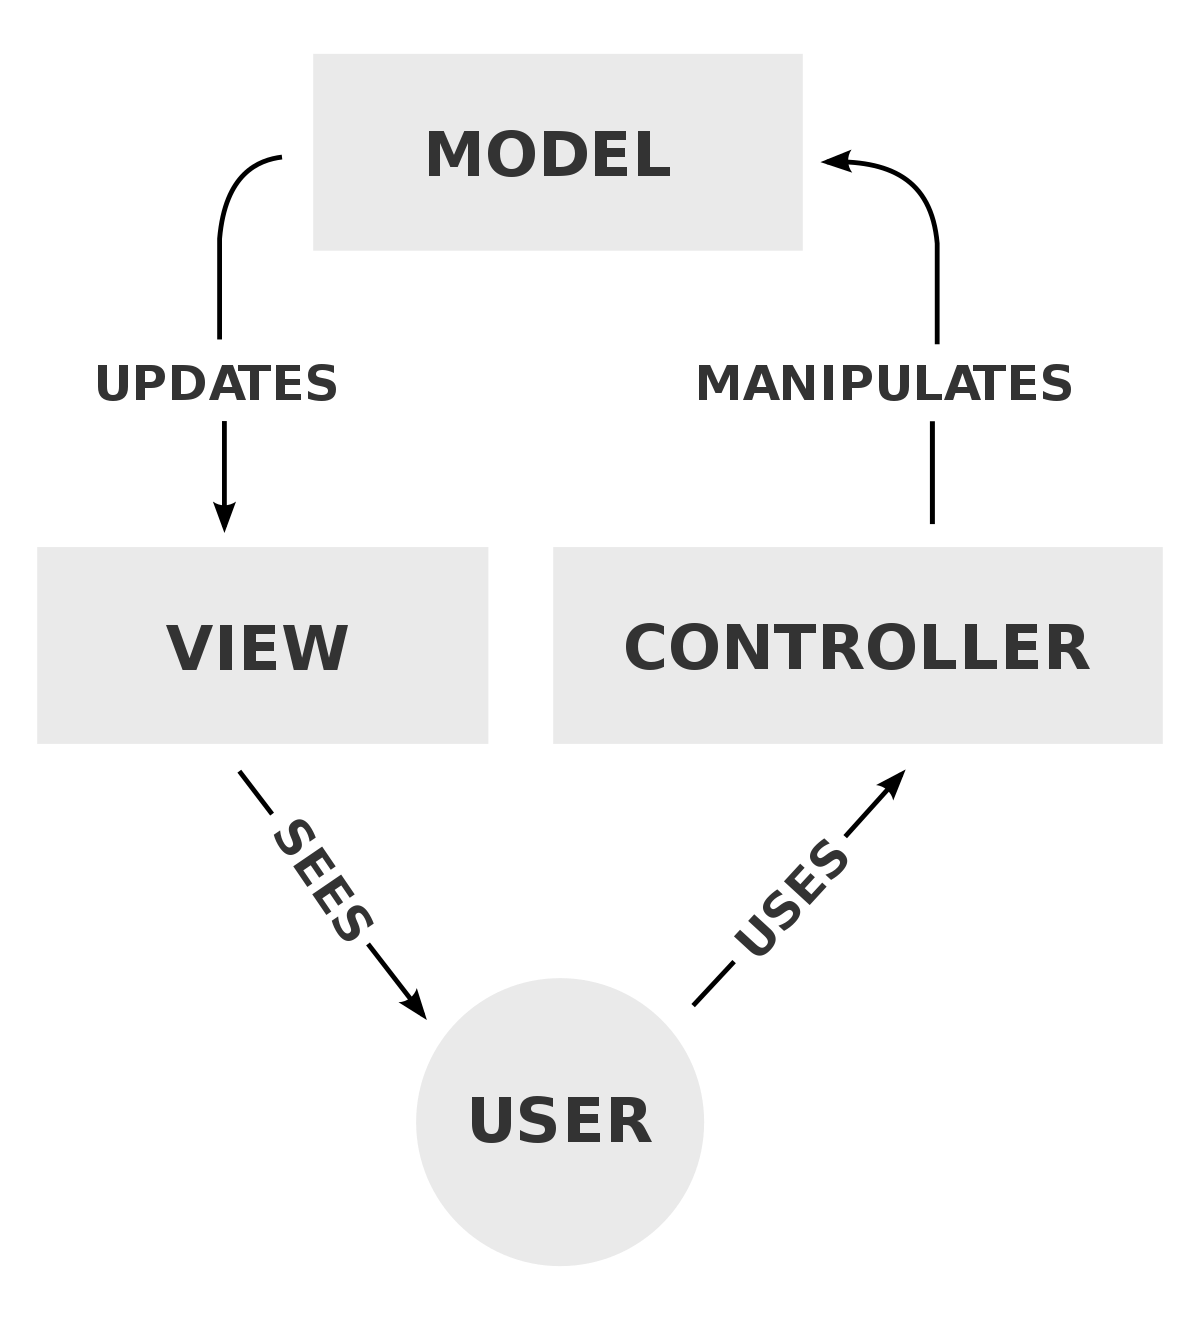
\includegraphics[width=0.3\textwidth]{images/mvc.png}
  \caption{MVC Design Pattern \cite{mvc}}
\end{figure}

A model is the single, definitive source of information about the data. It contains the required fields and behaviours of the stored data and generally, each model maps to a single database table. The model component in the high-level domain diagram represents the Twitter Account API credentials and Twitter Campaigns. The Twitter Account API credentials model stores information about the Twitter Account with API access, including the username and the consumer keys and access tokens. The Twitter Campaign model includes a name, a description, and the file to be executed. The view component in the high-level domain model represents the dashboard and the column in the dashboard to display information about the models. The domain specific language acts as the controller, which the user interacts with to manipulate the model to update the view. A potential feature of the project utilising the model-view-controller architecture is scheduling, where the user creates a scheduled post through the domain specific language, which creates a scheduled post in the model which displays in the view.

\section{Grammar}

The grammar designs define the syntactical structure of the domain specific language. Designing the grammar is the initial step for understanding the structure of a program for the domain specific language and how it will interact with the Twitter API. The first step to achieve this is to write out all the actions that the domain specific language should achieve based on the requirements analysis. The domain specific language should provide the functionality to tweet, retweet, favourite, schedule and direct message and this can be translated directly into a grammar rule `action'. \newline \par

The interaction of the Twitter API requires a RESTful service using JSON objects. An intuitive design approach for the domain specific language is to create a language with actions that generate JSON templates and values which populate the JSON object. An initial grammar design is inspired by and replicates a similar grammatical structure to JSON objects, where each action has a parameter with a key-value pair. The first grammar design, presented in extended Backus–Naur form (EBNF):

\begin{grammar}
<twitbot> ::= <statement `;'>+

<statement> ::= <action> <parameter> `,' <parameter>*

<action> ::= `tweet' 
\alt `retweet'
\alt `favourite'
\alt `schedule'
\alt `direct-message'

<parameter> ::= <identifier> `:' <value>

<identifier> ::= <string>

<value> ::= <string>

<string> ::= [a-zA-Z0-9]+
\end{grammar}

The initial grammar design is an extremely lightweight grammar as it has vasts amount of flexibility and is error-prone. This initial design of the grammar has limited and restricted functionality and power. The grammar does not include any conditional statements, types, looping or recursion. \newline \par

The first grammar does not directly represent an interaction with the Twitter API. The grammar is designed to populate JSON objects and does not provide any functionality for automation. The next design decisions evaluate the trade-offs of implementing this functionality through back-end software or extending the language further to include new features. This decision is prevalent while dealing with user authentication. For each Twitter API call a user must be authenticated. This authentication requires the user access tokens and consumer keys to be included in each Twitter API call. The current grammar design uses actions which represents a Twitter API call, and this requires each action grammar rule to include access tokens and consumer keys. A solution to this problem is to define macros in the language to retrieve user login credentials from a separate file to abstract the authentication from the user and increase code-reuse. Another solution to this is to utilise back-end software to manage the user authentication and abstract this from the user. As the requirements specify that it is mandatory for the domain specific language to be used by both programmers and non-programmers, utilising the power of back-end software keeps the language concise without adding any complexity. As the requirements analysis and the overall aims and objectives of the project are to include a web-application, the web-application will handle the management of authentication keys and tokens. \newline \par

The initial grammar lacks the majority of functionality specified in the requirements analysis, and its syntactical structure does not closely align with the problem domain. The next stage for grammar designs is to extend the actions further, splitting each action to have required and optional parameters, with the key-value pairs of these parameters encapsulating the logic of a Twitter API call. A program for the domain specific language should reflect a Twitter campaign, which allows for a list of actions to be performed and automated bot actions. An example of a Twitter Campaign for a brand is to market a new product. The program must reflect the logic of the different elements that go into a marketing campaign. This logic includes the scheduling of tweets, tweeting with images, retweeting and responding to mentions based on keywords. This leads to the final grammar design, which encapsulates the logic of having multiple tailored actions to perform different tasks. The final grammar design is presented in extended Backus–Naur form (EBNF) in appendix A.
\chapter{Implementation}

The implementation of the project is broken down into three distinct underlying components which all interact with each other. The first component is the implementation and execution of the domain specific language and the interpreter. The second component is the implementation of the interaction with the Twitter API. The third component is the web-framework which acts as a container for the interaction with the domain specific language and the front-end capabilities.

\section{ANTLR}

The first stage of implementation is to implement the domain specific language using ANTLR 4. ANTLR (ANother Tool for Language Recognition) is a powerful parser generator for reading, processing, executing, or translating structured text or binary files \cite{antlr}. ANTLR is widely used to build languages, so it is an obvious choice when deciding which tool to use to implement the domain specific language. \newline \par

The translation of the grammar designs to ANTLR implementation is a simple process. ANTLR has a syntax closely aligned with the standard notation for grammars. The design of the grammar is in extended Backus–Naur form (EBNF). Backus–Naur form is a notation technique for context-free grammars, which is used to describe the syntax of a language. Extended Backus-Naur form uses regular expressions repetition operators such as * and +. The basic form of an EBNF rule is: $a : b;$ and describes that symbol a on the left side can be replaced with the symbol b on the right side \cite{standard1996ebnf}.\newline \par

To generate a lexer and parser, ANTLR uses a context-free grammar expressed using EBNF to generate the parse-tree data structure. The use of EBNFs do not distinguish between lexer and parser rules and focuses on terminal and non-terminal symbols. In practice, terminal symbols are recognised by a lexer, and a parser recognises non-terminal symbols. ANTLR imposes this convention in which lexer rules start with an uppercase letter and parser rules with a lowercase letter. Lexer rules contain only references to other lexer rules or literals and parser rules may reference parser and lexer rules and include literals. ANTLR allows for the separation of the parser and lexer rules. The grammar in the project is split into parser rules dsl.g4, and the lexer rules dslLexerGrammar.g4 and NumericLexer.g4. \newline \par

The generated ANTLR parser uses LL(*) for parsing. An LL(*) parser, \textbf{L}eft-to-right, \textbf{L}eftmost derivation is a top down-parser that is not restricted by a finite number of tokens of lookahead and performs grammar analysis dynamically at runtime. An LL(*) parser is a natural extension to LL(K) parsers which make parsing decisions using at most $k$ symbols of lookahead, as LL(*) parsers can scan arbitrarily far ahead \cite{bovet2008antlrworks}. The parser can calculate how to recognise the sequences by appropriately iterating through the grammar as the parser has access to input sequences. This differs from static analysis, which has to consider infinitely long input sequences \cite{parr2011ll}. ANTLR 4 automatically re-writes self-referential rules that are left-recursive into non-left-recursive equivalents. Left-recursion in parsing often leads to infinite recursion in top-down parsers. \newline \par

Once ANTLR has generated a parser and a parse-tree, ANTLR provides tree walkers to visit the nodes of the parse trees, which can then execute application-specific code. In the context of the project, when the action nodes are visited, other nodes are then visited to extract data regarding the parsed input text. This process can be done automatically through the use of listeners or manually through the use of visitors.

\subsection{Listeners and Visitors}

ANTLR provides support for two tree-walking mechanisms in its runtime library. The parse tree listener interface is the default which is triggered by the built-in tree-walker. ANTLR generates a ParseTreeListener subclass specific to each grammar rule with enter and exit functions. The walker automatically performs a depth-first walk, and when the walker encounters the node for each rule, it triggers the enter and exit functions for the given rule. This mechanism is automatic and does not require a written parse-tree walker, and the listener methods do not have to visit their children explicitly \cite{parr2013definitive}.

\begin{figure}[!h]
  \centering
  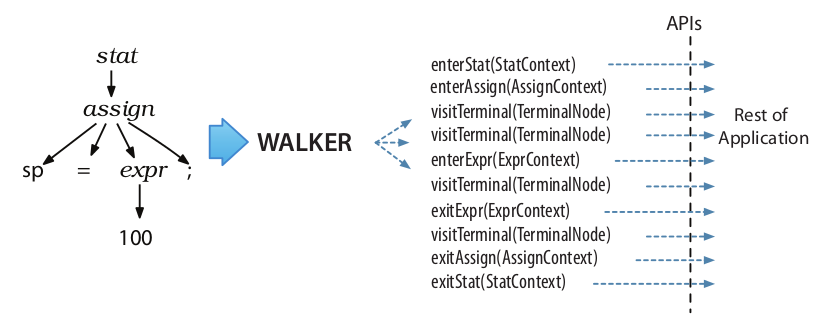
\includegraphics[width=0.8\textwidth]{images/antlrlistener.png}
  \caption{Sequence of calls made to the listener by ParseTreeWalker \cite{parr2013definitive}}
\end{figure}

The other mechanism for tree-walking is for ANTLR to generate a visitor interface from the grammar. This interface generates a visit method for each rule, and the walker performs a depth-first walk of the tree. The walk is initiated by application-specific code to create a visitor implementation and call the visit function. The generated visitor interface contains default implementations for the visitor methods. The visitor interface avoids having to override every method and can focus on the methods of interest \cite{parr2013definitive}. \newline \par

\begin{figure}[H]
  \centering
  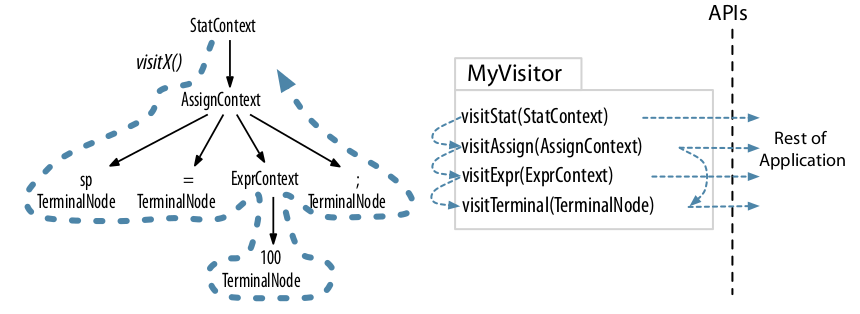
\includegraphics[width=0.8\textwidth]{images/antlrvisitors.png}
  \caption{Visitor pattern \cite{parr2013definitive}}
\end{figure}

The decided implementation of the tree-walking mechanism is the visitor interface. This implementation is in the `DSLVisitorWalker' class in `dslVistorWalker.py'. This mechanism was decided as it provides more control over the traversal of the tree. It allows the explicit call of the child nodes and retrieves the input values of the language based on the action node. This flexibility allows the walker only to have to visit the nodes which are needed. Visitor mechanisms also allow the function to return values, which is practical when testing. \newline \par

The Visitor mechanism allows for full control of the traversal of the tree, and acts as the interpreter for the system by executing application-specific code based on each action. The visitor mechanism differs from the Listener mechanism, which automatically visits every node and reacts to each node individually.

\section{Tweepy}

The second stage of implementation is to implement a way to interact with the Twitter API. The original design of the program to interact with the Twitter API was to build and create a RESTful web service. This original design of the RESTful web service is incredibly intricate and deals with low-level functionality including HTTP requests, authentication and rate limits. This implementation is time-consuming, prone to error and outside the scope of the project. The Tweepy package is a convenient way to access the Twitter API with Python, as it includes a set of classes and methods that represent Twitter's models and API endpoints. Tweepy handles implementation details such as \cite{api}:
\begin{itemize}
    \item Data encoding and decoding
    \item HTTP requests
    \item Results pagination
    \item OAuth authentication
    \item Rate limits
    \item Streams
\end{itemize}
Tweepy provides a simple way to interact and provide full functionality of the Twitter API. Using Tweepy allows more resources to be focused on the main scope of the project, to design, implement and focus on the functionality of the domain specific language without much concern as to how to interact with the Twitter API. \newline \par

The initial implementation of the Tweepy API is in `execute.py'. Tweepy supports OAuth 1a (application-user), which is required to interact with the Twitter API. The Execute class provides a function `tweepy\_auth()' which uses the consumer keys to generate an OAuthHandler, which is used to authenticate and access a Tweepy API object. \newline \par

The Tweepy API object is then passed to the DSLVisitorWalker, which is used to execute application-specific code. Based on each action, the relevant input information is retrieved and stored in kwargs, and kwargs allows the passing of keyworded variable length of named arguments to a function \cite{args}. Since the grammar of the domain specific language is closely aligned with the Twitter API, the key-value pairs in kwargs are the parameter name and parameter value. Using kwargs allows for the Visitor method to dynamically get all the required and optional parameters and pass kwargs to the correct Tweepy API call based on the action. This method of implementation provides a much simpler way to interact with the Twitter API than building a RESTful service. \newline \par

As Tweepy is a Python library, it provides a lot more functionality than interacting directly with the native Twitter API. Tweepy provides different objects such as Status objects, User objects and provides a Twitter Stream which retrieves tweets in real-time. The combination of these objects, StreamListeners and native Python, allows for a much more comprehensive range of possibilities for automation than the native Twitter API. The implementation of these features is demonstrated through Twitter Bots.

\subsection{Twitter Bots}

 This functionality is implemented in `bot\_scripts', which uses the Tweepy object to perform three different automation tasks. Utilising the Tweepy library allows for a simple solution for implementing bot scripts. An alternative would have been to have this functionality built into the domain specific language with program constructs such as looping and recursion. This method of implementation would have added complexity to the language which does not satisfy the needs of a novice user.
 
 \subsubsection{Reply to Mentions}
 
The first automation task `replyMentions.py' takes keywords and a loop-time to respond to mentions for $x$ amount of time-based on the keywords. The function `execute' iterates until the sum of the initiated date-time, and loop-time is greater than or equal to the current date-time. The function retrieves the mentions every 30 seconds until the loop variant condition is satisfied. The function retrieves only new mentions from the initiated date-time and responds if the retrieved tweet text includes any of the keywords. The implementation is simple using the Tweepy library. It provides the functionality to get the most recent mentions, iterate over each tweet in the mention, retrieve the contents of the tweet and respond based on if the content includes a specified keyword.
 
 \subsubsection{Follow all Followers}
 
The class FollowFollowers in `followFollowers.py' is the most straightforward automation task. The function retrieves a list of all the user's followers, iterates over the list and checks if the user account follows the follower and then follows the follower if they do not.
 
\subsubsection{Favourite Retweet Listener}
 
The class FavRetweetListener in `favRetweetListener.py' extends the tweepy.StreamListener class. StreamListener is used to retrieve tweets in real-time. Specific keywords filter the StreamLister, and individual actions can be performed based on the tweets it retrieves \cite{api}. In this bot script, it checks if the tweet does not belong to the user's account and if the tweet is not already tweeted or favourites, then it performs these actions. This automated task provides the ability for users to engage with large amounts of specified content automatically.

\section{Django}

Django is a Python-based free and open-source web framework that follows the model-view-template (MVT) architectural pattern. The model-view-template is a slightly different version to the traditional model-view-controller architecture, as Django controls the interactions between the Model and the View. This results in a template which is a HTML file mixed with Django Template Language. \newline \par

The execution of the domain specific language and interacting with the Tweepy API does not require Django. Django acts as a container, providing a simple and intuitive way to interact with the domain specific language. The interaction between Django and the domain specific language is through Django custom management commands. Django comes with a variety of command-line utilities that can be invoked and provides the functionality for custom commands. Custom management commands provides a simple way to interact with the application via command line. \newline \par

The custom management command used to interact with the domain specific language is `execute\_dsl.py', which takes two arguments, account\_id and campaign\_id. Django automatically produces an id field for every Model, and these are the arguments to be passed to the management command. The Models can be created through the Django admin site. The Django admin site is an automatic admin interface, which reads metadata from the models to provide a quick, model-centric interface where trusted users can manage content for the web application. The use of the Django management site is a temporary solution until the web application interface is implemented, which will provide the tools for a user to upload and execute the domain specific language. \newline \par

Using Django provides a simple solution for storing information about the Twitter Account, Twitter Campaigns and executing the domain specific language. Django also provides a testing-suite which uses the standard Python unittest module. The testing suite in Django provides a simple solution for writing and executing unit tests to test the complex and intricate aspects of the domain specific language.

\section{Execute Class}

The Execute class in `execute.py' provides the core functionality of the project as the class directly interacts with the domain specific language as it builds the parser, parses the input and initiates the tree traversal. The class also provides functions to retrieve the API credentials based on if they are stored in the TwitterAccount models or have been passed through as a parameter. This function is used to authorise and create the Tweepy object. The class can be executed by `execute\_dsl.py', which interacts with the class through the management command. Unit tests can execute the execute class by passing through an input statement and Twitter API credentials.

\section{Schedule Class}

The Schedule class in `schedule.py' provides the implementation and functionality of scheduling. The class takes schedule\_date\_time\_parameters, action, api, account and campaign parameters. The schedule\_date\_time\_parameters parameter is a dictionary containing all of the relevant information to schedule at a specific time. The action parameter is the remaining action to be executed by the domain specific language. These values have been derived from the dslVisitorWalker by traversing the parse tree and retrieving the values from the child nodes of the schedule action. The schedule function creates a DateTime object and calculates the total seconds between the time scheduled and the DateTime of the local machine. The upper limit of the scheduling time is the maximum stored number in an int value in seconds. The function uses a native Python scheduler `sched', which takes as parameters a time delay, priority, function to execute and arguments. The function to execute is the execute function, which builds the lexer and parser and traverses the tree, and this is executed at the specific date-time provided in the domain specific language.
\chapter{Evaluation}

The evaluation of the system is determined from a set of unit tests. The unit tests are split into four different classes which test different components and functionality of the system. The first class of unit tests, DSLParsingTest, tests how the input is parsed and if the visitor/interpreter implementation successfully visits the child nodes to return the correct input data. DSLParsingTest uses a different visitor class than the rest of the system, as this testing visitor class, DSLVisitorWalkerTest, returns the kwargs of the parsed input instead of executing application specific code. The kwargs are the result of the parsed input, which is to be passed to the Tweepy object to perform the actions of the given input. This testing class validates the core functionality of the domain specific language, the parser and the interpreter by proving the output is as expected for a valid input. \newline \par

The second test class, DSLVisitorWalkerAPITests, tests the visitor and the visitors interaction with the Twitter API through the Tweepy library. The test class tests all the core functionality and the different actions performed by the domain specific language. The unit tests directly interact with Twitter, making it difficult to control all the variables for unit testing. The tests can be run individually; however, running the test class is better suited as some test functions depend on other test functions. An example of this would be test\_retweet and test\_favourite as the unit tests would fail if ran twice with quick succession. This is because there would likely be no new tweets from the user's timeline, and the unit tests would throw an assertion error as the retrieved tweet would already be retweeted and favourited. \newline \par

The unit test class utilises the Tweepy library by interacting with a timeline tweet and assessing if the action functionality has been performed through assertions. Unit test functions such as test\_tweet perform an action and retrieve data from the timeline and check the text with a unique message to determine if the action has been performed correctly. The test class also tests the scheduling functionality. The function performs an assertion that the latest tweet text is not equal to the scheduled tweet text, executes the scheduling task, executes a delay of 60 seconds and then asserts the latest tweet text is equal to the input action text. \newline \par

The third test class, BotScriptTest, tests the bot scripts. These tests are not in the standard unit test form as it is an intricate task to assess their functionality in a unit test. This is due to the amount of unpredictable factors which involve the interaction of other Twitter accounts. An example of this would be the follow\_followers\_bot. Without other accounts API access, it is impossible to perform a unit test as selected accounts cannot follow and unfollow to determine if the bot has successfully achieved its functionality. These tests require user interaction to determine if they are functioning as intended. This requires a user to manually follow the bot account and check if the bot automatically follows the account when the test class or unit test has run. This applies to the other two bot scripts, where user interaction with other accounts is required to ensure the bots are working as intended. \newline \par

The final test class, TwitterAccountCampaignUploadTest, tests the functionality of uploads and execution using the Django models. It uses `test\_utils' to create Django Model objects and uploads a domain specific language program to be executed. The test class evaluates the functionality of executing a domain specific language through the use of text files. The other test classes test through the use of input strings as parameters. The TwitterAccountCampaignUploadTest class tests the majority of the functionality demonstrated in the other three classes. The test class does not test the functionality of the action `tweetImage' as uploading and asserting images in a unit test is a complex task. This functionality has been tested externally to ensure it executes as intended. \newline \par

The unit tests determine that the system works as intended with a syntactically correct input. It explores all functionality with different inputs to ensure each component of the system works correctly and interacts with the Twitter API as intended. The unit tests determine that Functional Requirement 1, 2, 3, 4 are all successfully achieved, meeting all the mandatory functional requirements. \newline \par

The unit tests do not explore the edge cases or when a syntactically invalid user input is entered. The unit tests could be extended further to test this functionality, and understand what happens when a syntactically incorrect input is entered. This includes inputs which are correct for the lexical analysis stage, but do not grammatically make sense and inputs which do not adhere to the grammar. The domain specific language does not perform any error handling. This is because ANTLR handles all error handling for parsing. Error messages are displayed to the user if the input is incorrect and the program terminates, which is a difficult task to encapsulate in unit testing. The unit tests could enter syntactically invalid programs and test that the raised errors are the ones expected to be generated by ANTLR. Completing these additional tests would allow the unit tests to prove the system can be interacted fully as intended and safe for practical application. 





\chapter{Summary and Reflections}

\section{Further Work}

Further extensions of the project would have been to include the functionality described in the desirable functional requirements. This includes implementing a front-end to the Django web application where users can interact with the domain specific language from a multi-user web page. The desirable functional requirements were not achieved due to time constraints and the complexity of the implementation of the system. \newline \par

Another extension of the project would be to include more automation and bot-scripts. The Tweepy API has powerful functionality which can be seen in the StreamListeners. StreamListeners obtains high volumes of tweets in real time and its functionality is demonstrated in FavRetweetListener in bot\_scripts. This functionality provides a lot of opportunities for automation and could be integrated with sentiment analysis in natural language processing to engage and interact with tweets based on its sentiment. There is vast potential for more complex and practical bot scripts to be implemented using the Tweepy API. \newline \par
 
The project meets Functional Requirement 1, as it provides all the functionality of what can be completed by a human on the standard web page. A limitation of this functional requirement is that the interaction of the basic functionality of Twitter is a complicated process. This is due to the Twitter API using Snowflake to generate unique IDs for objects within Twitter (Tweets, Direct Messages, Users). These ID's are often unknown and are not a viable or practical solution to interacting with the basic functionality of the API. Tweeting a user can manually be achieved by including their username following the standard \@ notation however to retweet, reply to tweet and favourite, the ID of the Tweet must be known. Further extensions of the project would look at solutions to solving this, including algorithms to search for ID's by usernames through the Tweepy API to create a more intuitive and natural interaction with the domain specific language.

\section{Conclusion}

The project was completed using an Agile SCRUM methodology. This methodology focuses on using short work cycles called sprints. Sprints throughout the project varied in length depending on what the sprint aimed to achieve in the sprint plan. The sprint plans used the GANT chart produced in the interim report to further break down tasks. This process of dividing the larger tasks into smaller sprint plans allowed for easy implementation of the project and was managed through a Trello board. This board included three columns, things to do, doing and completed. Each task within the column had a label and a sprint number to make it easy to identify which sprint cycle includes which tasks and what work is outstanding at the end of a sprint. This method of project planning was extremely effective, allowing each task to be easily managed and implemented and allowed for real-world delays and issues. The project timeline and management did not encounter many delays. The most significant delay for the management of the project was getting access to the Twitter API keys. It took several weeks to gain access to the keys and this delayed the implementation of the project as the application to gain access to the keys was not done until after the planning and designs. This delayed the implementation stage of the project as the API keys were vital for the implementation stage. \newline \par

The project was unable to meet the desirable requirements due to the underestimated amount of time it would take to successfully implement the domain specific language and the visitors. These limitations came from small amount of errors in the domain specific language which had to be refactored. Another factor was the choice to write the software in Python. ANTLR4 has Python 3 as a code generation target, but does not include any documentation for Python. This required all of the examples and documentation from The Definitive ANTLR 4 \cite{parr2013definitive} to be converted from Java to Python. This made implementation a slow process as the documentation and examples did not always directly translate to Python. In these scenarios it was required to view the ANTLR 4 Python source code to understand how to implement certain functionality and this was most prevalent when implementing the visitor functions. \newline \par

Other decisions to use certain tools and technologies added complications to the project. The decision to use the Python ANTLR generation was to use be able to easily include the domain specific language in the Django web application. As the front end of the Django web application was not implemented, it was not necessary to use Django. Django provides a simple way to manage the account credentials, execute the domain specific language, create Twitter Campaigns and execute tests. This is a nice feature and would work well with the future aims and objects and desirable requirements however for the project these features could easily be implemented without the use of Django. \newline \par

The original project ideas and designs had the intention of working across a wider range of social media platforms and not limited to Twitter. This project limitation came from the lack of access for the API and developer tools for other social media platforms. Other social media platforms such as Facebook and Instagram have limited access to their API and developer toolkits, where the specification of the project was not eligible for API access. \newline \par

\addcontentsline{toc}{chapter}{Bibliography}
\bibliographystyle{acm}
\bibliography{bibliography/bibliography}


\setlength{\grammarparsep}{2pt plus 1pt minus 1pt} % increase separation between rules
\setlength{\grammarindent}{15em} % increase separation between LHS/RHS

\begin{appendices}

\chapter{Final Grammar Design in EBNF}

\begin{grammar}
<twitbot> ::= (<statement> `;')+ 

<statement> ::= <action> 

<action> ::= <tweet>
\alt <tweetImage>
\alt <reply>
\alt <retweet>
\alt <favourite>
\alt <scheduleTweet>
\alt <directMessage>
\alt <autoFavouriteRetweet>
\alt <autoFollowFollowers>
\alt <autoReplyMentions>

<tweet> ::= `tweet' <tweet_req_param> \newline (`,' <tweet_optional_params>)*

<tweet_req_param> ::= `status' `:' <string>

<tweet_optional_params> ::= `possibly_sensitive' `:' <boolean>
\alt `lat' `:' <number>
\alt `long' `:' <number>
\alt `display_coordinates' `:' <boolean>

<tweetImage> ::= `tweet_image' <tweet_req_param> \newline `,' <tweetImage_req_param> \newline (`,' <tweet_optional_params>)*

<tweetImage_req_param> ::= `image_name' `:' <string>

<reply> ::= `reply_to_tweet' <reply_req_params> \newline (`,' <tweetImage_req_param>)? \newline (`,' <tweet_optional_params>)*

<reply_req_params> ::= `in_reply_to_status_id' `:' <number> `,' \newline `status' `:' <string>

<retweet> ::= `retweet' `id' `:' <number>

<favourite> ::= `favourite' `id' `:' <number>

<scheduleTweet> ::= `schedule' <scheduleTweet_req_param>

<scheduleTweet_req_param> ::= <date_time_param> `,' (<tweet> \alt <tweetImage>)

<date_time_param> ::= <minute> `,' <hour> `,' <day_of_month> `,' <month>

<minute> ::= `minute' `:' <numeric_minute>

<hour> ::= `hour' `:' <numeric_hour>

<day_of_month> ::= `day_of_month' `:' <numeric_day>

<month> ::= `month' `:' <numeric_month>

<directMessage> ::= `direct_message' <directMessage_req_params>

<directMessage_req_params> ::= `recipient_id' `:' <number> `,' `text' `:' <string>

<autoFavouriteRetweet> ::= `auto_fav_retweet' <keyword> (`,' <keyword>)* 

<autoFollowFollowers> ::= `follow_all_followers'

<autoReplyMentions> ::= `automate_reply_to_mentions' \newline <automateReply_req_param> (`,' <keyword>)+

<automateReply_req_param> ::= `automate_time_minutes' `:' <numeric_minute> `,' \newline `response' `:' <string>

<string> ::= [a-zA-Z0-9]+

<keyword> ::= `keyword' `:' <string>

<number> ::= <unary_operator>? <unsigned_number>

<unary_operator> ::= `+' \alt `-'

<unsigned_number> ::= <unsigned_int>
\alt <unsigned_float>

<unsigned_int> ::= (<digit>)+

<unsigned_float> ::= (<digit>)+ '.' (<digit>)*

<digit> ::= [0-9]

<boolean> ::= `True'
\alt `False'

<numeric_month> ::= 0[1-9]\alt1[0-2]

<numeric_day> ::= 0[1-9]\alt1[0-9]\alt2[0-9]\alt3[0-1]

<numeric_hour> ::= 0[0-9]\alt1[0-9]\alt2[0-3]

<numeric_minute> ::= 0[0-9]\alt1[0-9]\alt2[0-9]\alt3[0-9]\alt4[0-9]\alt5[0-9]

\end{grammar}

\end{appendices}


\end{document}